\icode{N16-MI-SI-L3-261109-003}
\nceeID[6]{2016新课标\Rmnum{3}}{17}
如图，两个轻环\(a\)和\(b\)套在位于竖直面内的一段固定圆弧上：一细线穿过两轻环，其两端各系一质量为\(m\)的小球，在\(a\)和\(b\)之间的细线上悬挂一小物块。平衡时，\(a\)、\(b\)间的距离恰好等于圆弧的半径。不计所有摩擦，小物块的质量为\paren[]

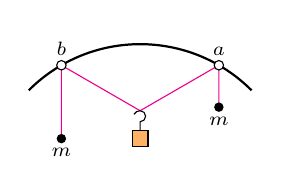
\begin{tikzpicture}[font=\scriptsize]
	\coordinate (A) at(0,{2*sqrt(3)/3});
	\draw[thick] (45:2) arc(45:135:2);
	\draw[magenta] (-1,.8)--(120:2)--(A)--(60:2)--(1,1.2);
	\fill (-1,.8)node[below]{\(m\)} circle(.06) (1,1.2)node[below]{\(m\)} circle(.06);
	\draw[fill=white] (60:2)node[above]{\(a\)} circle(.06) (120:2)node[above]{\(b\)} circle(.06);
	\draw (A) arc(90:-90:.07)--(0,.9) (A) arc(90:150:.09);
	\draw[fill=orange!60] (-.1,.9) rectangle(.1,.7);
\end{tikzpicture}
\begin{choices}
	\item\(\frac{m}{2}\)
	\item\(\frac{\sqrt{3}}{2}m\)
	\item\(m\)
	\item\(2m\)
\end{choices}
\begin{answer}
	C\qquad 提示：
\end{answer}